\chapter{Développement d'application}

Comme expliqué dans l'introduction chapitre ~\ref{chap:intro} le premier objective du stage était le développement d'applications de réalité augmentée spatiale.Il était important pour commencer le stage d'évaluer les possibilités offertes mais aussi les contraintes posés par le kit de développement. Le travail demandé ne se cantonnais donc pas uniquement au développement d'application mais il était important d'effectuer un travail d'analyse et de critique du kit.

\section{ReARTable}
D'après le contexte et le public ciblé par l'entreprise, il m'a paru intéressant de développer une démonstration au but à la fois ludique et éducatif. J'ai donc choisit de recréer la technologie Reactable\cite{reactable} proposé par la société du même nom.

La Reactable est un instrument de musique électronique permettant la génération de son en direct développé depuis 2003. Présenté sous forme d'une table interactive, le son est généré via des éléments tangibles (fig. ~\ref{fig:reactelem}) placés a sa surface. 

\begin{figure}[H]
\centering
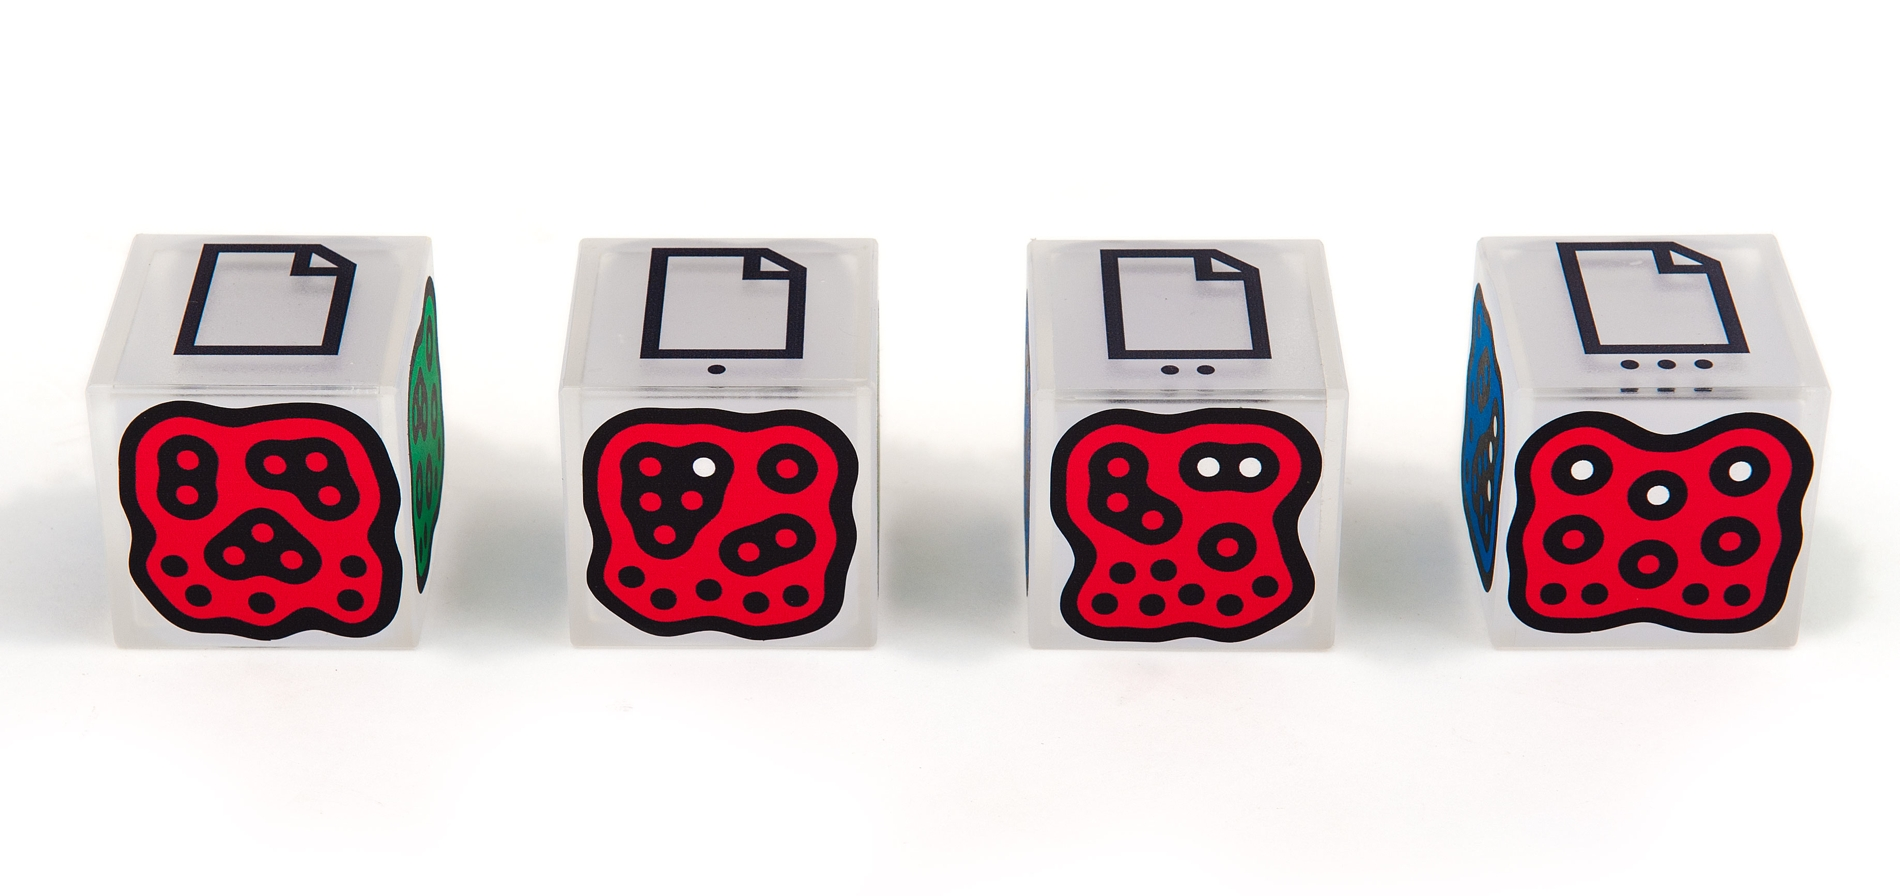
\includegraphics[width=0.6\textwidth]{images/reactelements}
\caption{Élément tangible utilisé pour la génération d'un élément de synthétiseur sur la Reactable\protect\footnotemark}
\label{fig:reactelem}
\end{figure}

\footnotetext{Source: \href{http://a-blok.com/FR/reactable.html}{Reactable : Elements tangibles}}

Chaque élément tangible représente un élément de synthétiseur qu'il est possible de contrôle de plusieurs façon:
\begin{itemize} 
\item La distance de l'élément par rapport a un autre élément. Cette propriété peut être utilisée pour contrôler, par exemple, l'interaction entre deux éléments.
\item L'orientation de l'élément sur la table. Cette propriété peut être utilisé pour contrôler, par exemple, la fréquence de l'élément ce qui va avoir pour effet par exemple pour un battement de ralentir ou d'accélérer ce dernier.
\item La disposition de l'élément. Cette propriété permet entre autre de combiner des éléments pour créer des nouveaux son plus riches et plus complexes.
\item La position du doigt de l'utilisateur par rapport a un élément. On peut venir contrôler divers paramètre comme l'amplitude par exemple en venant faire graviter son doigt autour d'un élément.
\end{itemize}
Ainsi, c'est en combinant plusieurs éléments entre eux avec différentes orientation et différentes dispositions que l'utilisateur va pouvoir peu a peu "construire" sa musique.
Au delà de la détection des éléments tangible, la table est rétro éclairée et permet donc la visualisation en directe de la musique générée (fig.~\ref{fig:reactivsu}).

\begin{figure}[H]
\centering
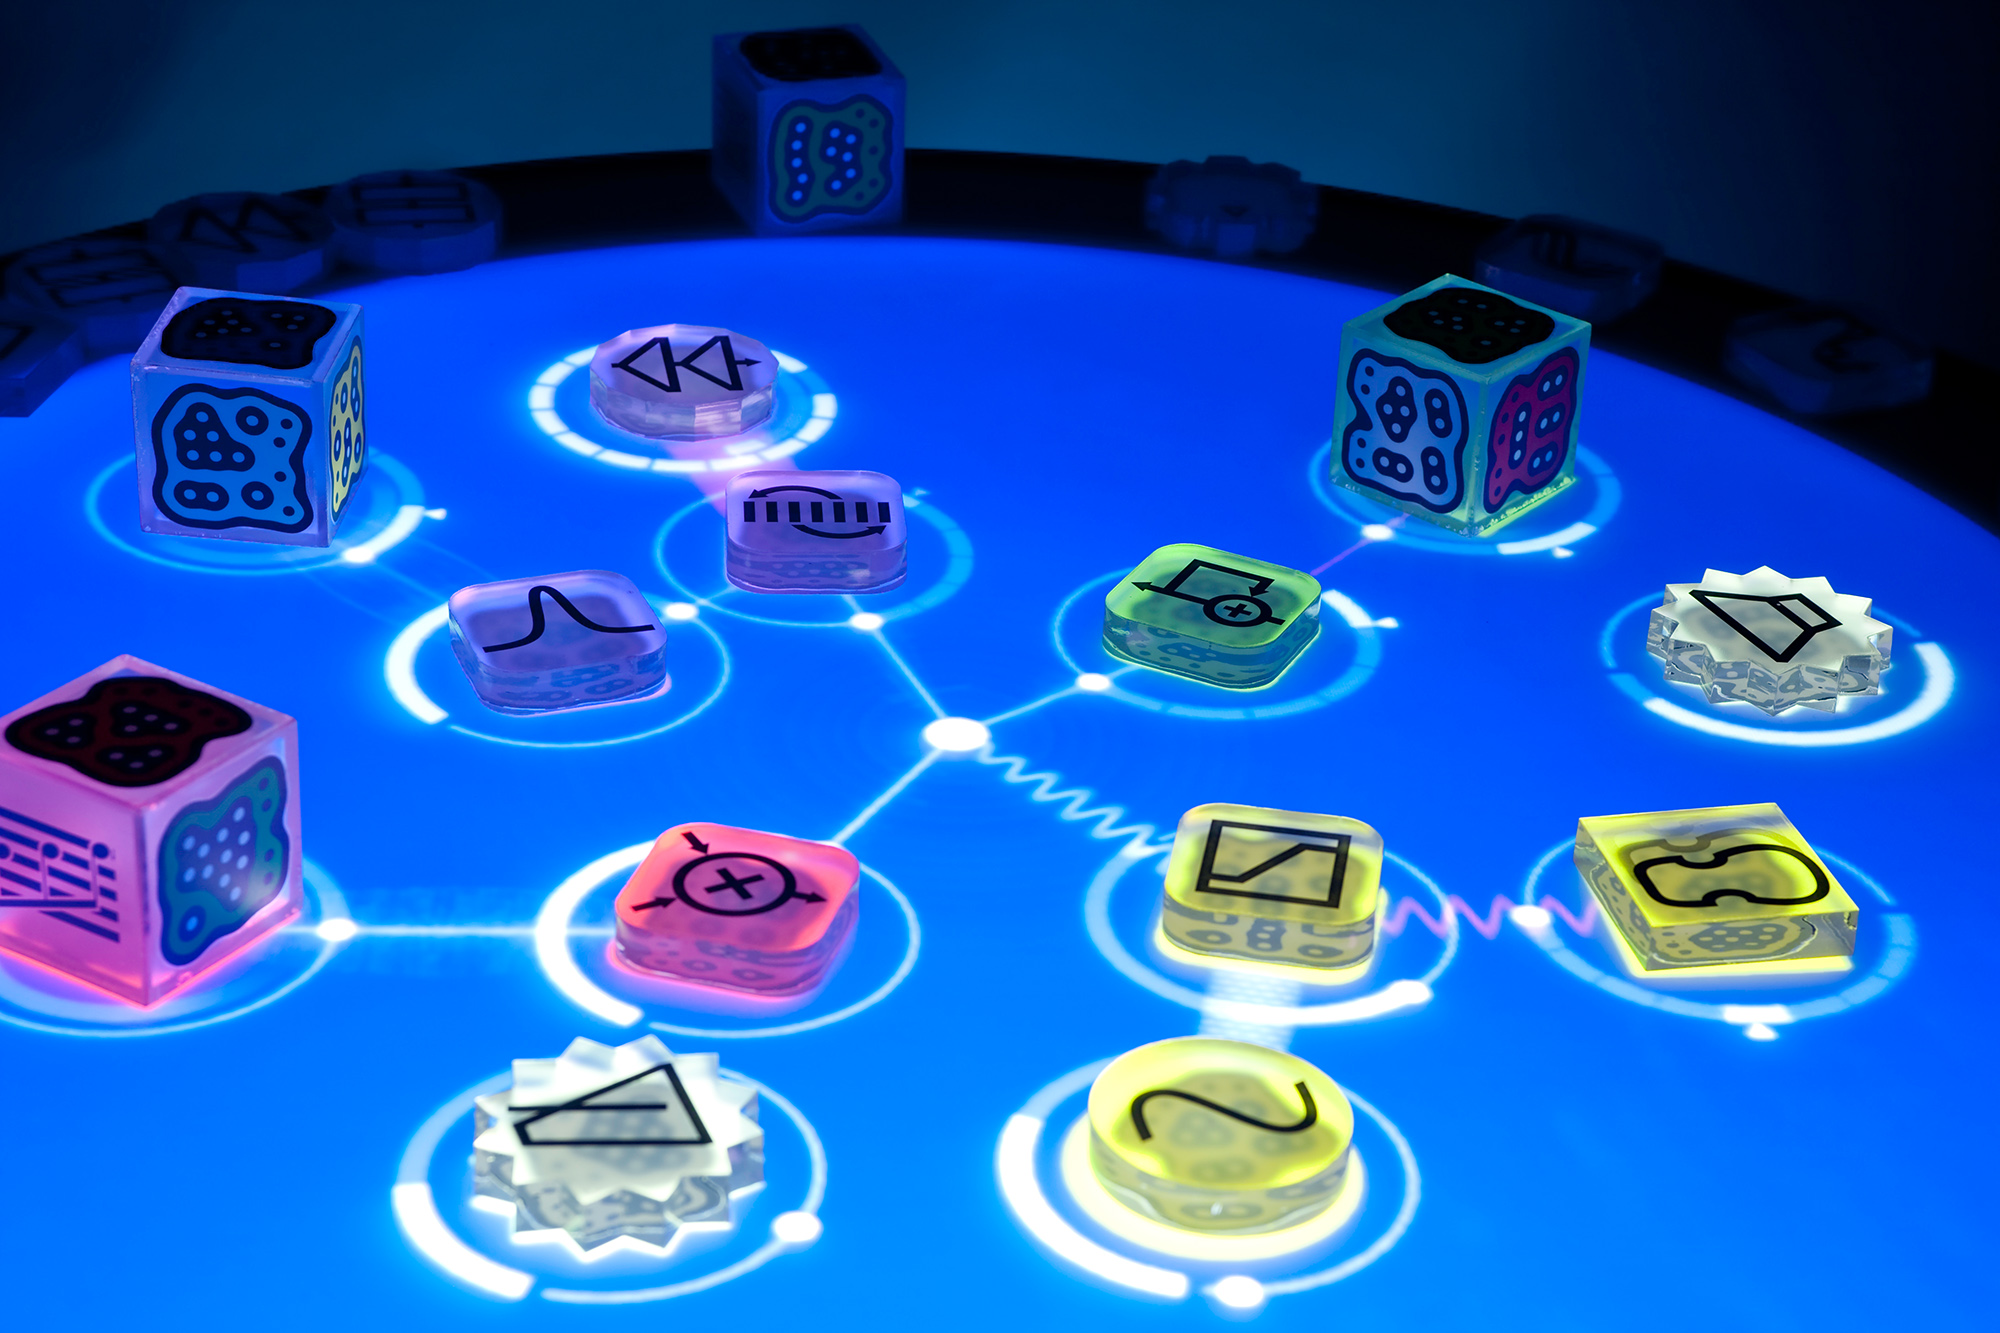
\includegraphics[width=0.65\textwidth]{images/reactvisu}
\caption{Visualisation du son sur la Reactable\protect\footnotemark}
\label{fig:reactivsu}
\end{figure}

\footnotetext{Source: \href{http://a-blok.com/FR/reactable.html}{Reactable}}


\subsection{Besoins et contenu de l'application}
Le but de l'application était de proposé une démonstration ce de qu'est capable de faire le système proposé par RealityTech et non pas de créer une application finie reprenant tous les points de la Reactable. Un tel développement pourrai faire l'objet d'un stage entier et ce n'était pas le cas ici.

Pour être en adéquation avec l'idéologie de l'entreprise, l'interface tangible et les modes d'interactions avec la musique était un point cruciale dans le développement de cette application.

Ainsi j'ai défini les besoins suivant pour l'application:
\begin{itemize}
\item Créer un son. L'application devait pouvoir générer du son.
\item Créer une représentation physique du son. Chaque son devait avoir sa représentation physique, c'est à dire, son élément qui une fois posé dans le champ de vision de la caméra allé détecter le son.
\item Détecter et identifier les éléments représentation des sons. Pour pouvoir jouer le bon son en fonction d'un objet physique, il fallait que l'applcation soit capable de détecter et d'identifier l'élément en question.
\item Contrôler les paramètres d'un son. L'application devait pouvoir contrôler certains paramètre défini a l'avance du son généré comme par exemple la fréquence ou l'amplitude.
\item Créer une visualisation basic d'un son. L'application devait proposer une visualisation du son généré pour guider l'utilisateur dans son expérimentation.
\end{itemize}

\subsubsection{Choix et implémentation}
L'application a donc été développé sous Processing en utilisant PapARt pour la partie visualisation, détection et projection et Sonic Pi\footnotetext{\href{https://sonic-pi.net/}{Sonic Pi site}} pour la génération de son.
Sonic Pi est un synthétiseur temps réel qui permet très facilement de générer des son cohérent. Le gros avantage de Sonic Pi est qu'il gère en interne énormément de problèmes posé par la génération dynamique de musique comme par exemple la synchronisation des effets, la boucle, le mixage etc.

Comme on peut le voir sur le schéma explicatif (fig ~\ref{fig:reartable:generalscheme}), les éléments tangible représentant des sons se présentent sous forme de regroupement d'éléments rond de petite taille. On peut différencier deux sons en fonction du contenu du regroupement (nombre et position des éléments rouges comparé a ceux des éléments bleu).
Une fois l'élément tangible détecté et identifié, un message OSC\footnotetext{Le protocole OSC où OpenSoundControl est un format de transmission de donnée conçu pour le controle en temps réel} est envoyé a un serveur SonicPi préalablement démarré.

Pour ce qui est du contrôle du son, une zone autour du composant est défini dans laquelle soit un élément tangible, soit une interaction physique (avec le doigt) peut venir contrôler le son (fig.~\ref{fig:reartable:interactionzone}).

\begin{figure}[H]
\centering
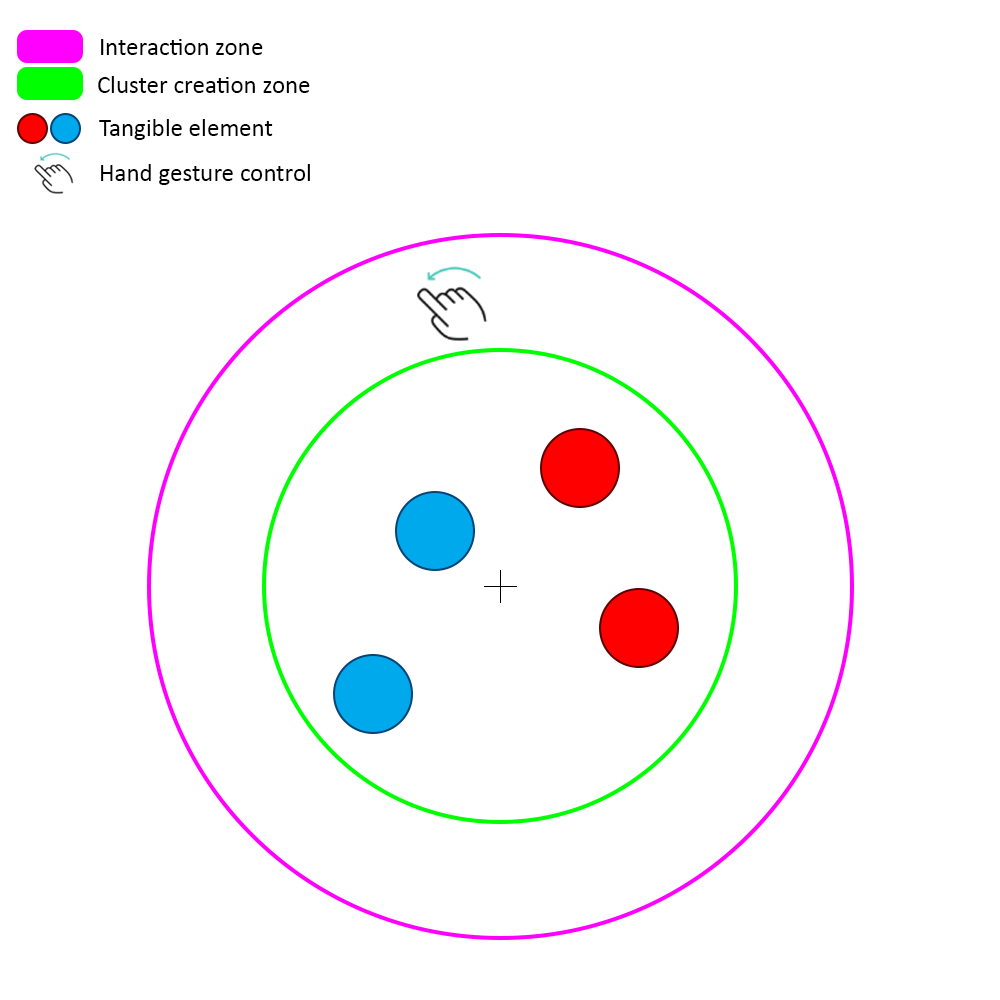
\includegraphics[width=0.65\textwidth]{images/reartable_cluster_interaction}
\end{figure}
% TODO Rajouter un petit schéma d'architecture de l'application avec Appli -> Message OSC -> Sonic Pi -> Génération de son et Sonic Pi -> Message OSC -> Appli -> Visualisation du son

% Analyse de technologie de la reactable
	% Retro eclairage -> marqueur fiduciaire -> interface tangible -> visualisation très poussés -> très cher
% Analyse rapide des besoins de l'application
	% Pouvoir créer différents effets sonores
	% Pouvoir jouer plusieurs effet sonores en même temps (cohérence des loops)
	% Apporter du controle aux effets sonores
	% Visualiser les effets sonores
	% Visualiser le son
% Proposition schématique de comment adapter la reactable au système actuel
% Proposition des modes d'interactions en adéquation avec le concept d'interface tangibles
% Parler de la visualisation (schéma expliquatifs)
% Parler du résultat final et des soucis d'implémentation
% Parler des cas d'utilisations

\section{Extraction de document}

% Analyse rapide des besoins de l'application
% Proposition schématique de toutes les techniques misent en oeuvre (expliquer la notion d'echelle et de connaissance a priori)
% Parler du résultat final et des soucis d'implémentation
% Parler des cas d'utilisation